\PassOptionsToPackage{quiet}{fontspec}
\documentclass[UTF8]{ctexart}

\usepackage[a4paper, total={6in, 8in}]{geometry}
\usepackage{amssymb}
\usepackage{graphicx}
\graphicspath{{./images/}}
\usepackage{listings}
\usepackage{hyperref}
\usepackage{multirow}
\usepackage{xcolor}
\usepackage{framed}

% adding commands

% a new command which severs arbitrary section number
\newcommand{\asection}[2]{
  \setcounter{section}{#1}
  \addtocounter{section}{-1}
  \section{#2}
}

\definecolor{code}{HTML}{dddddd}
\definecolor{codered}{HTML}{cc0200}
\definecolor{codepurple}{HTML}{cc33cc}
\definecolor{codegreen}{HTML}{519179}
\definecolor{codelavender}{HTML}{e1ecfe}

\newcommand{\acode}[1]{
  \colorbox{code}{\lstinline[basicstyle=\ttfamily]{#1}}
}
\newcommand{\acodered}[1]{
  \colorbox{codered}{\lstinline[basicstyle=\ttfamily\color{white}]{#1}}
}
\newcommand{\acodeppl}[1]{
  \colorbox{codepurple}{\lstinline[basicstyle=\ttfamily\color{white}]{#1}}
}
\newcommand{\acodegrn}[1]{
  \colorbox{codegreen}{\lstinline[basicstyle=\ttfamily\color{white}]{#1}}
}

\newenvironment{anote}{
  \colorlet{shadecolor}{codelavender}
  \begin{shaded}}
    {\end{shaded}}

\newenvironment{awarn}{
  \colorlet{shadecolor}{red!20}
  \begin{shaded}}
    {\end{shaded}}




\title{Practical MsSql}
\author{Jacob}
\date{2023-12-15}

\begin{document}
\maketitle

\section{概览}

目标与配置:

\begin{itemize}
	\item 目标:主备多地存储,故障转移。
	\item 配置:Ubuntu 22.04 LST,SQL Server 2022。
\end{itemize}

MsSql 集群部署知识:

\begin{itemize}
	\item MsSql 配置业务连续性
	\item Pacemaker 基础知识
\end{itemize}

\newpage
\section{MsSql}

\subsection{安装与启动}

\begin{lstlisting}[language=Bash]
	sudo apt-get update
	sudo apt-get install mssql-server mssql-server-ha

	sudo systemctl status mssql-server

	sudo systemctl start mssql-server
	sudo systemctl status mssql-server
\end{lstlisting}

\subsection{可用性的基础概念}

可用性种类:

\begin{itemize}
	\item 备份、还原
	\item 可用性组
	\item 故障转移集群
	\item 日志传送
\end{itemize}

可用性组(availability groups, AG)将数据库的每个事务发送到另一个实例或副本。AG 具有一个数据库的完全读/写副本,且位于主要副本上,所有次要副本都不能直接
从最终用户或应用程序接受事务。参与 AG 的实例可以是独立实例,也可以是故障转移集群实例(failover cluster instances, FCIs)。

AG 有一个名为侦听器的组件,该组件运行应用程序和最终用户在不知道哪个 SQL Server 实例为主要副本的情况下进行连接。每个 AG 都有自己的侦听器,实现可用性必须
具备 OS 层的基础集群。

\begin{figure}[ht]
	\centering
	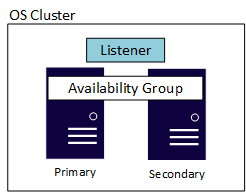
\includegraphics[width=0.5\textwidth]{{/simple-availability-group.png}}
\end{figure}

在可用性方面,AG 可提供自动(需要配置侦听器)或手动故障转移。

\begin{itemize}
	\item 在 Linux 上,AG 的所有故障转移(手动或自动)都是通过集群完成的。
	\item 在 Linux 上的 SQL Server,AG 建议配置至少三个副本。
	\item 在 Linux 上,每个侦听器使用的公用名都在 DNS 中定义。
\end{itemize}

\subsubsection*{可用性组集群类型}

微软为支持 Pacemaker 的 AG 和 FCI 配置(自动故障转移等)提供了\acode{mssql-server-ha}包,Pacemaker 中没有网络名称资源,该组件用于提取侦听器(或 FCI
名称)。DNS 在 Linux 上提供名称解析。

三种集群类型:

\begin{itemize}
	\item WSFC (Windows server Failover Cluster),该类型暂不考虑
	\item External (Linux),Linux 需要高可用的必选类型
	\item None
\end{itemize}

对于基于 Linux 的 AG,在创建 AG 时,集群类型必须设置为 External。

\subsubsection*{REQUIRED\_SYNCHRONIZED\_SECONDARIES\_TO\_COMMIT}

用于控制同步副本时发生的情况:

\begin{itemize}
	\item 三种值:\acode{0},\acode{1}与\acode{2}
	\item 值时必须同步的次要副本数,它对数据丢失、AG 可用性和故障转移都有影响
	\item 集群类型为 None,默认值为\acode{0},可手动设置\acode{1}或\acode{2}
	\item 集群类型为 External,默认值由集群机制设置,可手动重写;对于三个同步副本,默认值为\acode{1}
\end{itemize}

在 Linux 上,\acode{REQUIRED_SYNCHRONIZED_SECONDARIES_TO_COMMIT} 的值在群集中的 AG 资源上配置。

\acode{REQUIRED_SYNCHRONIZED_SECONDARIES_TO_COMMIT} 还影响故障转移行为,在 Linux 上,若该值为\acode{0}则不允许自动故障转移,因此必须大于\acode{0}。

\subsubsection*{安装 SQL Server 包以实现可用性}

对于 Linux 下的高可用性 SQL Server 实例,应使用 SQL Server 安装两个包:

\begin{itemize}
	\item SQL Server 代理(\acode{mssql-server-agent})
	\item 高可用性(HA)包(\acode{mssql-server-ha})
\end{itemize}

SQL Server 代理在 SQL Server 2017 CU4 及更高版本无需安装,直接启用即可。虽然 SQL Server 代理在技术上是可选的,但它是 SQL Server 的作业计划程序,并且
是日志传送所必需的,因此建议安装。启用方式 :

\begin{lstlisting}
	/opt/mssql/bin/mssql-conf set sqlagent.enabled true
	systemctl restart mssql-server
	/opt/mssql/bin/mssql-conf get sqlagent
\end{lstlisting}

\subsection{创建和配置可用性组}

流程:

\begin{enumerate}
	\item 部署 Pacemaker 高可用性集群。
	\item 启用可用性组。
	\item 创建可用性组终结点和证书。
	\item 使用 SQL Server Management Studio (SSMS) 或 Transact-SQL 创建可用性组。
	\item 为 Pacemaker 创建 SQL Server 登录和权限。
	\item 在 Pacemaker 集群中创建可用性组资源(External 类型)。
\end{enumerate}

\newpage
\section{Pacemaker}

\subsection{Pacemaker 基础知识}

Pacemaker 是一个高可用的集群资源管理器 -- 软件运行在若干节点的集群上,保持完整性和最大限度的减少所需服务的停机时间。Pacemaker 的关键特征有:

\begin{itemize}
	\item 节点层与服务层失败的发现与恢复
	\item 通过格栅错误节点来确保数据一致性
	\item 支持每个集群一个及以上的节点
	\item 支持多资源接口标准
	\item 支持共享存储(非必须)
	\item 支持冗余设置(主被动,N+1 等)
	\item 可以从任何节点更新的自动复制配置
	\item 能够指定服务间的集群范围的关系,例如排序、托管和反托管
	\item 支持高级服务类型,例如\textit{克隆}(需要在若干节点上可用的服务),\textit{可拓展克隆}(角色二选一的克隆),以及容器化服务
	\item 统一的可编写脚本的管理工具
\end{itemize}

\begin{anote}
	\textbf{格栅 Fencing}\bigskip

	\textit{格栅},又称为 STONITH(Shoot The Other Node In The Head),它确保了节点不可能运行服务的能力。通过\textit{格栅设备},例如只能电源开关或切断
	目标对本地网络访问的只能网络交换机等,来完成的。

	Pacemaker 将格栅设备视为一类特殊的资源。

	如果没有格栅,集群就无法从某些特定故障条件中安全恢复,例如无响应节点。
\end{anote}

集群架构:

\begin{itemize}
	\item \textbf{资源}
	\item \textbf{资源代理}
	\item \textbf{格栅代理}
	\item \textbf{集群成员层}
	\item \textbf{集群资源管理器}
	\item \textbf{集群工具}
\end{itemize}

\subsection{安装与启动}

% TODO

\subsection{创建集群}

% TODO

\end{document}
